\documentclass[12pt, letterpaper]{extarticle}

\usepackage{geometry}
\usepackage{graphicx}
\usepackage{setspace}
\usepackage[T1]{fontenc}
\usepackage{lmodern}
\usepackage{amsmath}
\usepackage{amssymb}
\usepackage[spanish]{babel}
\usepackage{csquotes}
\usepackage[hidelinks]{hyperref}
\usepackage[shortlabels]{enumitem}
\usepackage{mathtools}
\usepackage{array}
\usepackage{subfiles}

\geometry{left=1in, bottom=1in, right=1in, top=1in}

\graphicspath{{Media}}

\newcommand{\newSection}[1]{\section*{#1}\addcontentsline{toc}{section}{#1}}
\newcommand{\newSubSection}[1]{\subsection*{#1}\addcontentsline{toc}{subsection}{#1}}
\newcommand{\newSubSubSection}[1]{\subsubsection*{#1}\addcontentsline{toc}{subsubsection}{#1}}
\newcommand{\unit}[1]{\ensuremath{\; \mathrm{#1}}}

\begin{document}

\subfile{Portada.tex}

\newpage

\tableofcontents

\newpage

\newSection{Diseño de embragues y frenos}

\newSubSection{Introducción}

Se llama freno a todo dispositivo capaz de modificar el estado de movimiento de un sistema mecánico mediante fricción, pudiendo incluso detenerlo completamente, absorbiendo la energía cinética de sus componentes y transformándolo en energía térmica. El freno está revestido con un material resistente al calor que no se desgasta con facilidad, no se alisa y no se vuelve resbaladizo.

Una representación dinámica simplificada de un embrague o freno de fricción se muestra e nla siguiente figura. Dos inercias, $I_{1}$ e $I_{2}$, que viajan respectivamente a velocidades angulares $\omega_{1}$ y $\omega_{2}$, de las que una puede ser cero en el caso de los frenos, y se llevan a la misma velocidad al hacer la conexión del embrague o freno.

\begin{figure}[h]
    \centering
    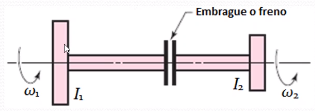
\includegraphics[width=0.5\textwidth]{Media/dinamica_simp_freno.png}
    \caption{Representación dinámica de un embrague o freno.}
    \label{Fig: Representacion dinamica de un embrague o freno}
\end{figure}

El par de torsión que se transmite se relaciona con la fuerza de accionamiento, el coeficiente de fricción y la geometría del embrague o freno.

Los diversos tipos de dispositivos (embragues y frenos) se clasifican de la manera siguiente:
\begin{itemize}
    \item De aro (tambor) con zapatas internas expansibles.
    \item De aro (tambor) con zapatas externas contráctiles.
    \item De banda.
    \item De disco o de tipo axial.
    \item De tipo cónico.
\end{itemize}

\newSubSection{Análisis estático de embragues y frenos}

Se pueden analizar muchos tipos de embragues y frenos conforme un procedimiento general.

Dicho procedimiento comprende las siguientes tareas:
\begin{itemize}
    \item Se calcula, modela o mide la distribución de la presión en las superficies de presión.
    \item Se determina una relación entre la máxima presión y la presión en cualquier punto.
    \item Se emplean las condiciones del equilibro estático para obtener la fuerza de frenado o el par de torsión y las reacciones de los apoyos.
\end{itemize}

\end{document}